\chapter{مطالعه موردی فارسی}
\label{ch:casestudy}

\section{گراف دانش اسناد شهرداری}
\label{sec:municipality}

این فصل همان سامانه را بدون تغییر معماری روی داده فارسی اجرا می‌کند. چیزی که می‌خواستیم ببینیم این بود که آیا کاری که برای انگلیسی و دامنه عمومی ساخته شده، به یک زبان و دامنه دیگر منتقل می‌شود یا نه.

داده، اسناد واقع‌نمای شهرداری تهران است. آن را عمداً به‌هم‌پیوسته طراحی کردیم، یعنی یک موجودیت مثل «پروژه بهسازی پل صدر» یا یک ردیف بودجه، در چند سند مختلف و با نقش‌های متفاوت ظاهر می‌شود. جدول \ref{tab:muni} ابعادش را می‌دهد.

\begin{table}[ht]
\centering
\caption{ابعاد داده شهرداری و گراف حاصل از آن.}
\label{tab:muni}
\small
\begin{tabular}{|r|c|}
\hline
ویژگی & مقدار \\
\hline
سند منبع & $7$ \\
\hline
حجم متن خام & $811$ واژه \\
\hline
سه‌تایی خام با شاهد & $39$ \\
\hline
گره یکتا & $38$ \\
\hline
یال یکتا پس از ادغام & $32$ \\
\hline
نوع موجودیت & $6$ \\
\hline
نوع رابطه & $5$ \\
\hline
\end{tabular}
\end{table}

هستان‌شناسی این دامنه شش موجودیت دارد: پروژه، پیمانکار، مکان، مسئول، بودجه و شکایت. پنج رابطه هم میان آن‌ها تعریف شده است.

\section{نتیجه اجرا روی داده فارسی}
\label{sec:muni-result}

کل گراف را با متن منبع مقایسه کردیم و تمام رابطه‌های استخراج‌شده مورد تأیید متن بودند، یعنی چیزی نزدیک صد درصد. هیچ رابطه جعلی یا خارج از هستان‌شناسی به گراف نرسید. با کلیدگذاری بودجه بر پایه کد ثابت هم یک بودجه که در چند سند با نام‌های متفاوت آمده بود، به یک گره واحد نگاشت شد. شکل \ref{fig:muni} نمای گراف و شکل \ref{fig:muni-ev} نمونه ردیابی یک رابطه تا جمله منبع را نشان می‌دهد.

\begin{figure}[ht]
\centering
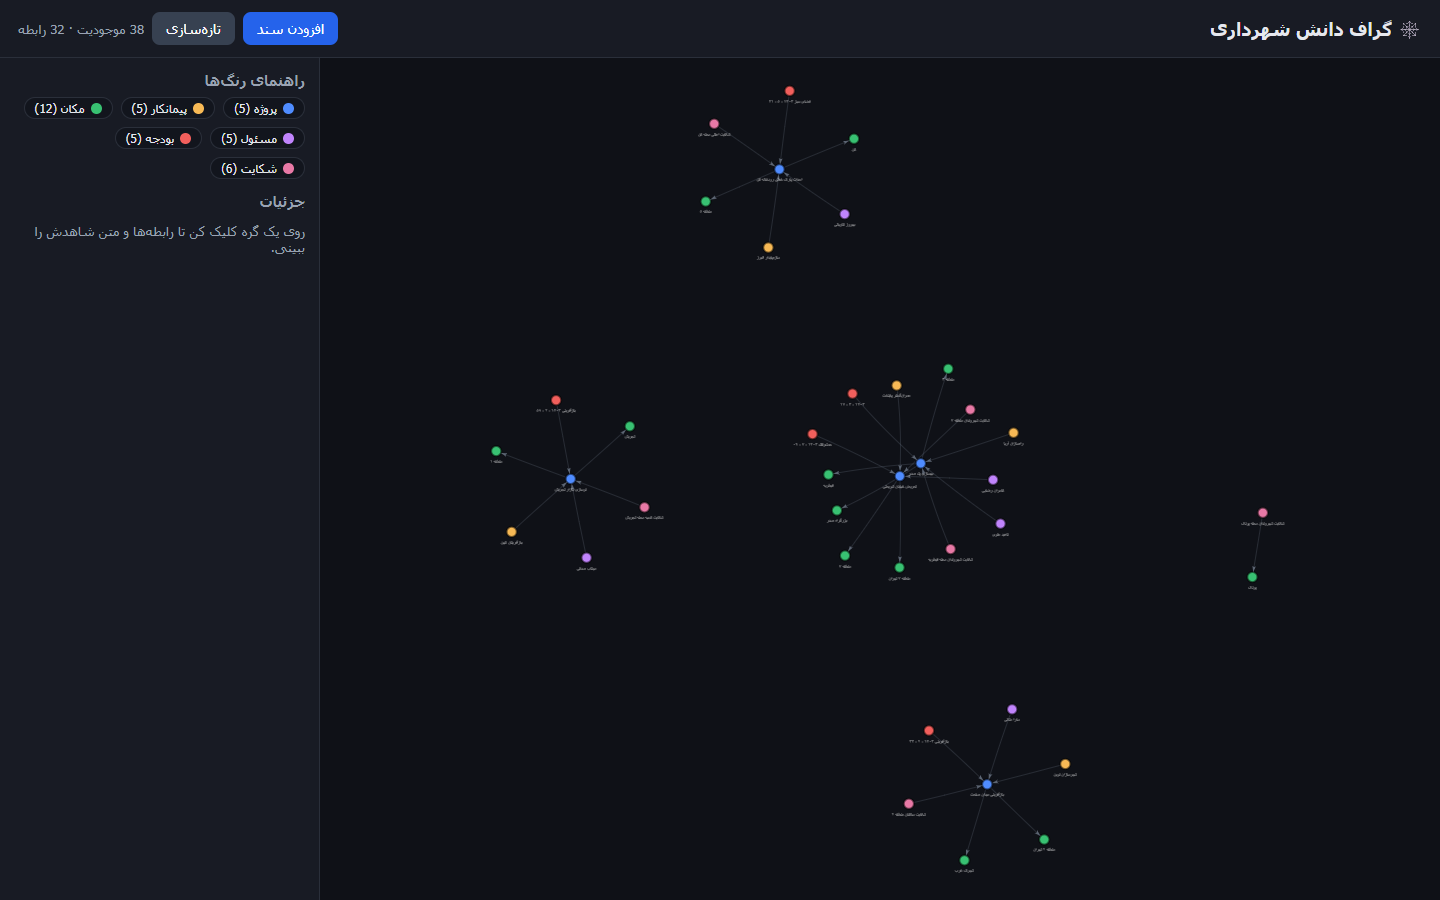
\includegraphics[width=0.9\textwidth]{Images/graph_output.png}
\caption{نمای کلی گراف دانش ساخته‌شده از هفت سند فارسی شهرداری.}
\label{fig:muni}
\end{figure}

\begin{figure}[ht]
\centering
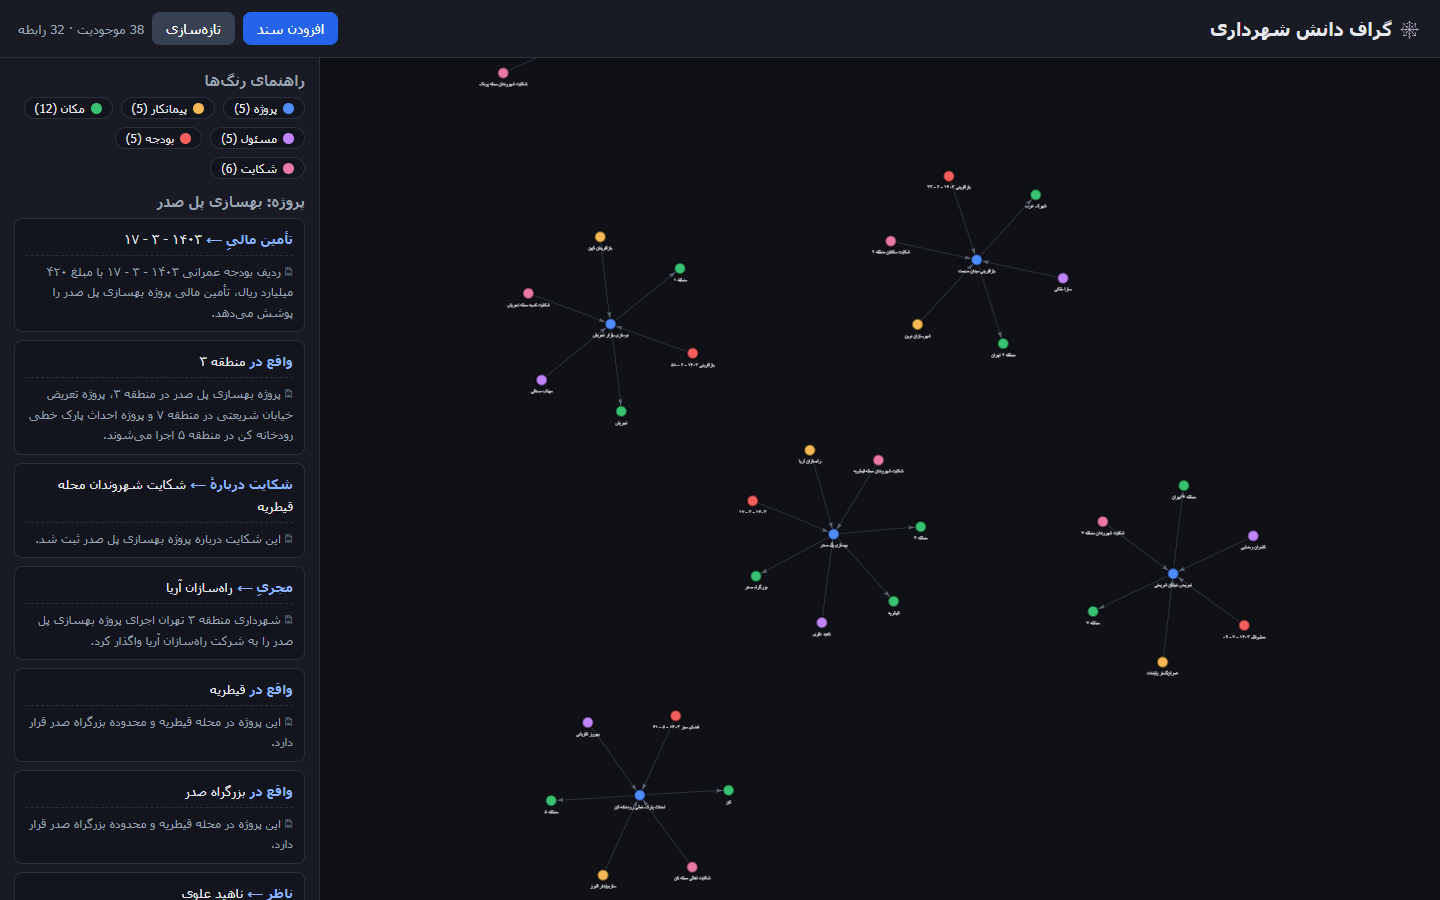
\includegraphics[width=0.9\textwidth]{Images/graph_evidence.png}
\caption{کلیک روی یک گره، رابطه‌های آن و جمله منبع هر رابطه را نشان می‌دهد.}
\label{fig:muni-ev}
\end{figure}

\section{چرا دقت اینجا صد درصد است و آنجا سی و پنج درصد}
\label{sec:why-gap}

وسوسه‌انگیز است که این تفاوت را به حساب بهتر کار کردن مدل روی فارسی بگذاریم، اما هیچ شاهدی برای چنین ادعایی نداریم. سه توضیح ساده‌تر وجود دارد.

نخست، فضای برچسب اینجا پنج رابطه دارد و آنجا نود و شش تا. وقتی مدل باید از میان پنج گزینه یکی را بردارد، احتمال انتخاب غلط طبیعتاً بسیار کمتر است.

دوم، و مهم‌تر از همه، ارزیابی اینجا دستی بود نه مبتنی بر برچسب طلایی. ما فقط می‌توانیم بگوییم هرچه استخراج شد درست بود؛ اینکه چه چیزهایی از قلم افتاد را اصلاً نمی‌دانیم. به بیان دقیق‌تر، آنچه اندازه گرفتیم دقت بود و نه بازخوانی.

سوم، اسناد شهرداری کوتاه و صریح‌اند و رابطه بین‌جمله‌ای در آن‌ها کم است، حال آنکه در \lr{Re-DocRED} بیش از نیمی از رابطه‌ها بین دو موجودیتی برقرارند که هرگز در یک جمله کنار هم نیامده‌اند.

همین مقایسه توضیح می‌دهد که چرا رفتن سراغ یک بنچمارک استاندارد ضروری بود: وقتی برچسب طلایی در کار نباشد، عدد دقت بیش از آنکه اطلاع بدهد، گمراه می‌کند.

سامانه در نهایت بدون اینکه معماری‌اش دست بخورد روی دو زبان، دو دامنه و دو هستان‌شناسی کار کرد که تعداد رابطه‌هایشان نوزده برابر با هم فرق دارد، و تنها چیزی که بین این دو اجرا عوض شد یک فایل \lr{JSON} بود. درسی که از این فصل گرفتیم این است که جدا نگه داشتن هستان‌شناسی از کد، تصمیمی که اولش فقط به چشم مرتب‌کاری می‌آمد، همان چیزی بود که انتقال‌پذیری را ممکن کرد.
